\documentclass[oneside, 12pt]{article}

\newcommand{\source}[1]{\textbf{Source:} {#1} }

\usepackage{indentfirst}
\usepackage{listings}
\usepackage{graphicx}
\usepackage{float}
\usepackage{color}
\usepackage{amsmath}
\usepackage[utf8]{inputenc}
\usepackage[english]{babel}
\usepackage[backend=bibtex]{biblatex}
\usepackage{color}
\usepackage{appendix}

\addbibresource{ref.bib}

\definecolor{pblue}{rgb}{0.13,0.13,1}
\definecolor{pgreen}{rgb}{0,0.5,0}
\definecolor{pred}{rgb}{0.9,0,0}
\definecolor{pgrey}{rgb}{0.46,0.45,0.48}

\usepackage{listings}
\lstset{language=Java,
  showspaces=false,
  showtabs=false,
  breaklines=true,
  showstringspaces=false,
  breakatwhitespace=true,
  commentstyle=\color{pgreen},
  keywordstyle=\color{pblue},
  stringstyle=\color{pred},
  basicstyle=\ttfamily,
  moredelim=[il][\textcolor{pgrey}]{\$\$},
  moredelim=[is][\textcolor{pgrey}]{\%\%}{\%\%}
}

\begin{document}
\title{Java 8 Parallel Streams}
\author{Ethan Williams}
\date{\today}
\maketitle

\tableofcontents

\setcounter{section}{-1}
\section{Prerequisites}

\subsection{Technical}
This document was written for Java developers who have an interest in using concurrency in streams, and assumes knowledge of serial streams and lambda expressions. Developers in other languages with similar mechanisms such as C\# with \verb|Linq| may also find the topics useful with the understanding that syntax, implementation, and functionality will differ.

Additionally, functional knowledge of \verb|java.util.concurrent| and the \verb|Consumer| interface will help in gaining a more practical knowledge but is not required.

\subsection{Vocabulary Clarification} \label{language}
Some of the vocabulary in the paper may be unfamiliar to those with a knowledge of streams and are defined/clarified below:
\begin{itemize}
\item A stream instantiated with the \verb|stream()| method only is referred to as a \textit{serial stream}
\item A stream instantiated with the \verb|parallel().stream()| or \verb|parallelStream()| methods is referred to as a \textit{parallel stream}
\item \textit{Serializing data} refers to destroying the stream and bringing all collection items left in the stream into memory
\item A stream is composed of 3 parts: a source which is the \verb|Collection| it is operating on, intermediate operations such as \verb|map()| which don't serialize data, and terminal operations like \verb|toArray()| which serialize the stream
\end{itemize}

\section{Introduction}
Parallel streams were introduced into Java 8 alongside serial streams so that developers could utilize concurrency to make stream processing faster.  Concurrency allows the program to utilize threads in order to more efficiently utilize modern multiprocessor design. In the case of parallel streams, each thread handles a different part of the stream and assemble all the parts together when the stream is serialized \autocite{parallelism_doc}

Making a serial stream into a parallel stream is as easy as calling \verb|parallel()| after \verb|stream()|. In order for the \verb|parallel()| method to be applicable on the stream, the \verb|Collection| must have an implementation of a \verb|Spliterator| \autocite{ibm_uh_3}, an object which can effectively break up a collection to be processed separately. 

Several operations are more essential to parallel streams, as is the case with \verb|Collector|s. Calling the \verb|collect()| method on the stream which will reduce and serialize it based on the behavior of the \verb|Collector| object passed as an argument. With parallel streams, \verb|Collector|s are the recommended strategy for reduction because other mechanisms that can be used in serial streams will result in inconsistent results when run in parallel. The reason for this is discussed in Section \ref{stateful_expressions}.

Despite parallel streams being introduced into Java to simplify concurrency, developers can easily corrupt data and cause system bugs. Although there are a plethora of bugs that can arise from improper use of Java concurrency practices, there are several issues specific to the parallel stream implementation which are covered in this paper. This includes submitting long-running or blocking operations to a stream, interference with the source of the stream, and using stateful expressions.
\section{Spliterator}
The \verb|Spliterator| is the backbone of parallel streams, allowing the program to split a collection apart and iterate through it. If a class extending a \verb|Collection| does not have a \verb|spliterator()| method returning a \verb|Spliterator| object, then Java is not able to process the collection with a parallel stream at all.

{\itshape \verb|Spliterator| implementations differ based on the type of source collection, so this section focuses on a modified implementation for Java's \verb|ArrayList|}.

\subsection{Functionality}
A \verb|Spliterator| is an object which is represents the elements in a given range of the backing collection and represents the entire source collection at the beginning of a parallel stream. Calling the method \verb|trySplit()| will return a new \verb|Spliterator| that represents some subset of the original \verb|Spliterator|, while the original represents the rest of the collection. In the code example, the new \verb|Spliterator| represents first half of untraversed elements while modifying the instance to represent the second half of untraversed elements. Figure \ref{fig:split} illustrates a call to \verb|trySplit()| on a Spliterator representing the entire collection.

\begin{figure}[H]
\centering
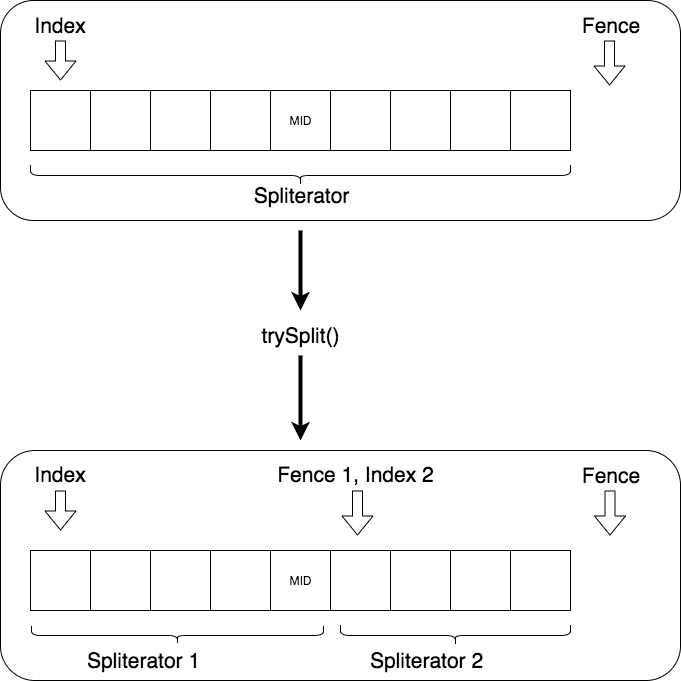
\includegraphics[width=8cm]{images/spliterator_illustrated.png}
\caption{A Spliterator Before and After Splitting}
\source{Ethan Williams}
\label{fig:split}
\end{figure}

\subsection{Implementation}
In the example implementation of \verb|Spliterator|, there are 3 instance fields: a source collection, an index, and a fence. The backing collection for each instance is the entire collection it is based on which ensures every instance has a consistent copy of the source. The index is the current cursor position of the \verb|Spliterator|, which is analogous to the cursor position in an Iterator object. The fence is the index of the last element the Spliterator is responsible for plus one. The primary methods used are \verb|tryEachRemaining()|, \verb|tryNext()|, \& \verb|trySplit()|. 

Although the cursor is similar to Iterator's, traversal through a Spliterator using \verb|tryEachRemaining()| and \verb|tryNext()| is different. \verb|tryEachRemaining()| in Figure \ref{fig:forEachRemaining} takes a Consumer object which is the operation to be executed on each element of the collection. A typical implementation will simply iterate through all elements and call the \verb|accept()| method on the consumer with the element as its only parameter. \verb|tryNext()| in Figure \ref{fig:tryAdvance} is similar although the operation is only attempted on element at the current cursor position. If that cursor position is past the fence of the Spliterator, then the method returns false, otherwise it returns true.

\begin{figure}[H]
\centering
\begin{lstlisting}[language=Java]
public void forEachRemaining(Consumer<? super E> action) {
    int i;
    if ((i = index) >= 0 && (index = fence) <= a.length) {
        for (; i < hi; ++i)  action.accept((E) list.elementData[i]);
    }
    throw new ConcurrentModificationException();
}
\end{lstlisting}
\caption{Implementation of forEachRemaining()}
\source{Java ArrayList, modified by Ethan Williams}
\label{fig:forEachRemaining}
\end{figure}

\begin{figure}[H]
\centering
\begin{lstlisting}[language=Java]
public boolean tryAdvance(Consumer<? super E> action) {
    int hi = getFence(), i = index;
    if (i < hi) {
        index = i + 1;
        action.accept((E) list.elementData[i]);
        return true;
    }
    return false;
}
\end{lstlisting}
\caption{Implementation of tryAdvance()}
\source{Java ArrayList, modified by Ethan Williams}
\label{fig:tryAdvance}
\end{figure}

\verb|Spliterator|'s primary functionality is encapsulated within the \verb|trySplit()| method in Figure \ref{fig:trySplit}. This method is called when the JVM wants to break the source collection in order to start processing the stream on another thread and if implemented incorrectly can be a subtle but important error in an application. The example implementation simply finds the midpoint and either returns a new \verb|Spliterator| from the cursor to the midpoint and the current instance of \verb|Spliterator| now covers mid to the fence. The example \verb|trySplit()| method is the code behind the split behavior illustrated in Figure \ref{fig:split}.

\begin{figure}[H]
\centering
\begin{lstlisting}[language=Java]
public Spliterator<E> trySplit() {
    int lo = index, mid = (lo + fence) >>> 1;
    return (lo >= mid) ? null : new Spliterator<E>(list, lo, index = mid);
}
\end{lstlisting}
\caption{Implementation of trySplit()}
\source{Java ArrayList, modified by Ethan Williams}
\label{fig:trySplit}
\end{figure}

\section{Collector}
A \verb|Collector| object defines a mutable reduction operation for a group of input elements and is used in a stream with the \verb|collect()| method. In other words, instances reduce a stream into a data structure which may be different than the source. To utilize \verb|Collector|s in streams, developers can either use one of the many methods of the \verb|Collectors| class such as \verb|averagingInt()|, \verb|groupingByConcurrent()|, and many more. Alternatively, a developer may choose to write their own \verb|Collector| to reduce the stream differently.

\subsection{Functionality}
%NEW INTO SENTENCE
The example shown in Figure \ref{fig:employee_collection} groups employees by department into a \verb|Map| object with the department as the key and a list of employees in that department as a value. \verb|Collector|s can be used on both serial and parallel streams, though using the general reduction function \verb|reduce()| is harder to use correctly with parallel streams since ordering is not guaranteed.

\begin{figure}[H]
\centering
\begin{lstlisting}[language=Java]
Map<Department, List<Employee>> byDept
    = employees.stream()
       .collect(Collectors.groupingBy(Employee::getDepartment));
\end{lstlisting}
\caption{Reduction of employees into map by a Collector}
\source{Ethan Williams}
\label{fig:employee_collection}
\end{figure}

\subsection{Implementation}

%REWRITE THIS WRT THE NEW FIGURE

A \verb|Collector| object has four methods which comprise the majority of its functionality: \verb|supplier()|, \verb|accumulator()|, \verb|combiner()|, \& \verb|finisher()| \autocite{collector_doc}. Figure \ref{collector} illustrates how all four methods work visually and are referred to in explanations below. Additionally, a code example in Figure \ref{fig:collector_impl} in Appendix A illustrates a basic implementation which reduces a stream into an \verb|ImmutableSet| and will also be explained below. 

The \verb|supplier()| method returns a mechanism to build an instance of a mutable data structure that will hold the elements of the stream which is known as the \textit{accumulator} \autocite{custom_collector}. Behind the scenes, the JVM will call this method several times to create \verb|ImmutableSet|s for all of the substreams.  In the code example our \verb|supplier()| is simply an \verb|ImmutableSet| builder so the JVM can generate new instances at will.

The \verb|accumulator()| method takes an accumulator and an element as parameters and will return a \verb|BiConsumer| object which details how the element should be added to the accumulator. The JVM uses this when of any element in the substream is done with processing to determine how or if it's added to the final data structure. In the code example, the \verb|accumulator| simply appends the element to the end of the \verb|ImmutableSet|.

%STOPPED HERE NEED TO REDO REST OF IMPLEMENTATION SECTION
The \verb|combiner()| method details the logic on how two accumulators should be joined together, which is simply appending right to left in the code example.  Funcionally, this is joining together two different \verb|ImmutableSets|.

Finally, the \verb|finisher()| method converts an accumulator into the resultant data type and returns it, finishing the reduction. In the code example, this is as easy as returning the built \verb|ImmutableSet|. 

\begin{figure}[H]
\centering
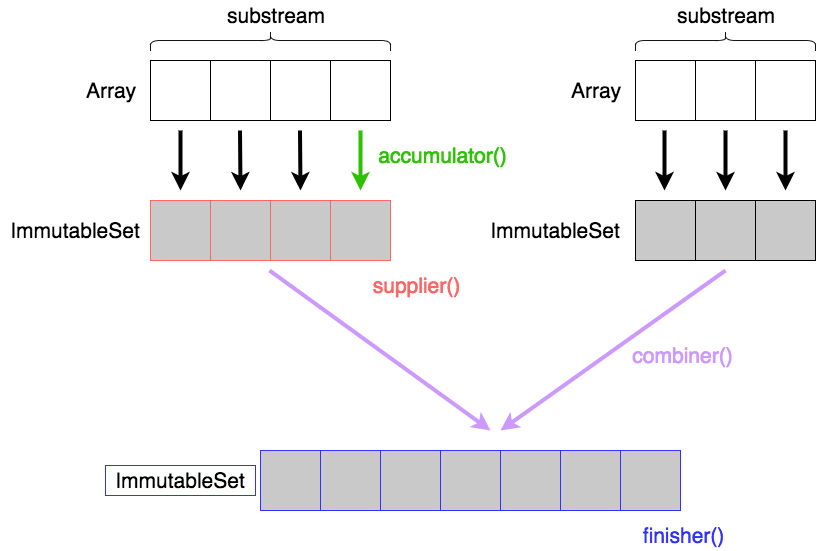
\includegraphics[width=13cm]{images/collector.png}
\caption{How a Collector is Used}
\source{Ethan Williams}
\label{fig:collector}
\end{figure}

\section{Practical Considerations when Using Parallel Streams}
Using parallel streams may seem easy but there are several common pitfalls for developers. Many of these errors arise from programmers not considering normal facets of concurrent programming such as submitting blocking or long-running tasks during execution. Additionally, some of the implementation details of parallel streams prohibit interference with the stream source and stateful expressions inside intermediate operations.

\subsection{Long-Running/Blocking Operations}
Mistakes that can arise from not knowing Java's implementation can have arguably more severe consequences on application performance. One example relates to how the JVM breaks a parallel stream into threads. When a parallel stream is processes, the JVM begins by processing on the calling thread. As more subtasks are broken off, the JVM gets threads from \verb|ForkJoinPool.common()|, which is a common thread pool used in the background of the whole application \autocite{dzone_dangers}. 

With the JVM's use of a common thread pool, one example of an error that could arise is if there is a long-running operation in a parallel stream as shown in Figure \ref{fig:network_op}. Each thread in the pool will be consumed executing that operation and subsequently all other JVM tasks using the common thread pool have to wait. This can lead to severe degradation in performance. Luckily, there is a way to fix this (or at least make it better).

\begin{figure}[H]
\centering
\begin{lstlisting}[language=Java]
Optional<String> result = collection.stream().parallel().map((base) -> longOperation(argument).findAny();
\end{lstlisting}
\caption{Reduction of employees into map by a Collector}
\source{Ethan Williams}
\label{fig:network_op}
\end{figure}

Although parallel streams can run into issues because it uses the common thread pool for the whole application, Java now allows a parallel stream to run with its own \verb|Thread Pool|. An example of how to implement this on the previous code snippet is shown in Figure \ref{fig:custom_pool}. This alleviates the issue because if one parallel stream is undermining performance, other parallel streams can still use threads even though the common pool doesn't have any more threads \autocite{dzone_fjp}.

\begin{figure}[H]
\centering
\begin{lstlisting}[language=Java]
ForkJoinPool customPool = new ForkJoinPool(4);
Optional<String> result = customPool.submit(() -> collection.stream().parallel().map((arg) -> longOperation(arg).findAny()).get();
\end{lstlisting}
\caption{Reduction of employees into map by a Collector with custom Thread Pool}
\source{Ethan Williams}
\label{fig:custom_pool}
\end{figure}

\subsection{Interference}
Editing the source of the stream in an intermediate operation will throw a \verb|ConcurrentModificationException| \autocite{parallelism_doc}. \verb|Stream|s do not contain any of the elements of the collection, instead they store references to the location of each element currently in the stream \autocite{ibm_uh_3}.  The stream in figure \ref{fig:interference} attempts to add each element to the collection again. Since it attempts to modify the source before the stream has serialized, this operation will throw a \verb|ConcurrentModificationException|.

\begin{figure}[H]
\centering
\begin{lstlisting}[language=Java]
collection.stream().parallel().map((x) -> collection.add(x)).toArray();
\end{lstlisting}
\caption{A stream which causes interference and will throw an error}
\source{Ethan Williams}
\label{fig:interference}
\end{figure}

\subsection{Stateful Expressions} \label{stateful_expressions}
The third practice which will cause errors in a stream and should be watched carefully is using stateful expressions in an intermediate operation. The code in Figure \ref{fig:stateful} shows an example of a stateful operation while attempting to add elements to \verb|parallelStorage| and print them. The issue is that although the \verb|forEachOrdered| method is just fine and will print in the expected order. \verb|parallelStorage|, however, will have a different ordering every time the stream is executed. The addition is stateful, meaning it depends on ordering and in parallel streams ordering can't be guaranteed in intermediate operations \autocite{parallelism_doc}.

\begin{figure}[H]
\centering
\begin{lstlisting}[language=Java]
List<String> parallelStorage = Collections.synchronizedList(new ArrayList<>());
collection.stream().parallel().map(x -> parallelSotrage.add(x)).forEachOrdered(x -> System.out.println(x));
\end{lstlisting}
\caption{A stream which causes interference and will throw an error}
\source{Ethan Williams}
\label{fig:stateful}
\end{figure}
 
\printbibliography[heading=bibintoc]

\appendix
\section{Code Example from Section 3.2}
\begin{figure}[H]
\centering
\begin{lstlisting}[language=Java]
import com.google.common.collect.ImmutableSet;
 
public class ImmutableSetCollector<T> 
        implements Collector<T, ImmutableSet.Builder<T>, ImmutableSet<T>> {
    @Override
    public Supplier<ImmutableSet.Builder<T>> supplier() {
        return ImmutableSet::builder;
    }
 
    @Override
    public BiConsumer<ImmutableSet.Builder<T>, T> accumulator() {
        return (builder, t) -> builder.add(t);
    }
 
    @Override
    public BinaryOperator<ImmutableSet.Builder<T>> combiner() {
        return (left, right) -> {
            left.addAll(right.build());
            return left;
        };
    }
 
    @Override
    public Function<ImmutableSet.Builder<T>, ImmutableSet<T>> finisher() {
        return ImmutableSet.Builder::build;
    }
 
    @Override
    public Set<Characteristics> characteristics() {
        return EnumSet.of(Characteristics.UNORDERED);
    }
}
\end{lstlisting}
\caption{Custom Collector }
\source{\autocite{custom_collector}}
\label{fig:collector_impl}
\end{figure}

\end{document}